\subsection{Training Dynamics}

After hyperparameter selection, the final ResNet-34 configuration is trained for 30 epochs using AdamW and cosine annealing learning rate scheduling. Training statistics are recorded using both local history logging and \texttt{wandb}, including epoch-level metrics, iteration-level loss, and learning rate evolution.

\begin{figure}[H]
    \centering
    
    \begin{subfigure}{0.4\textwidth}
        \centering
        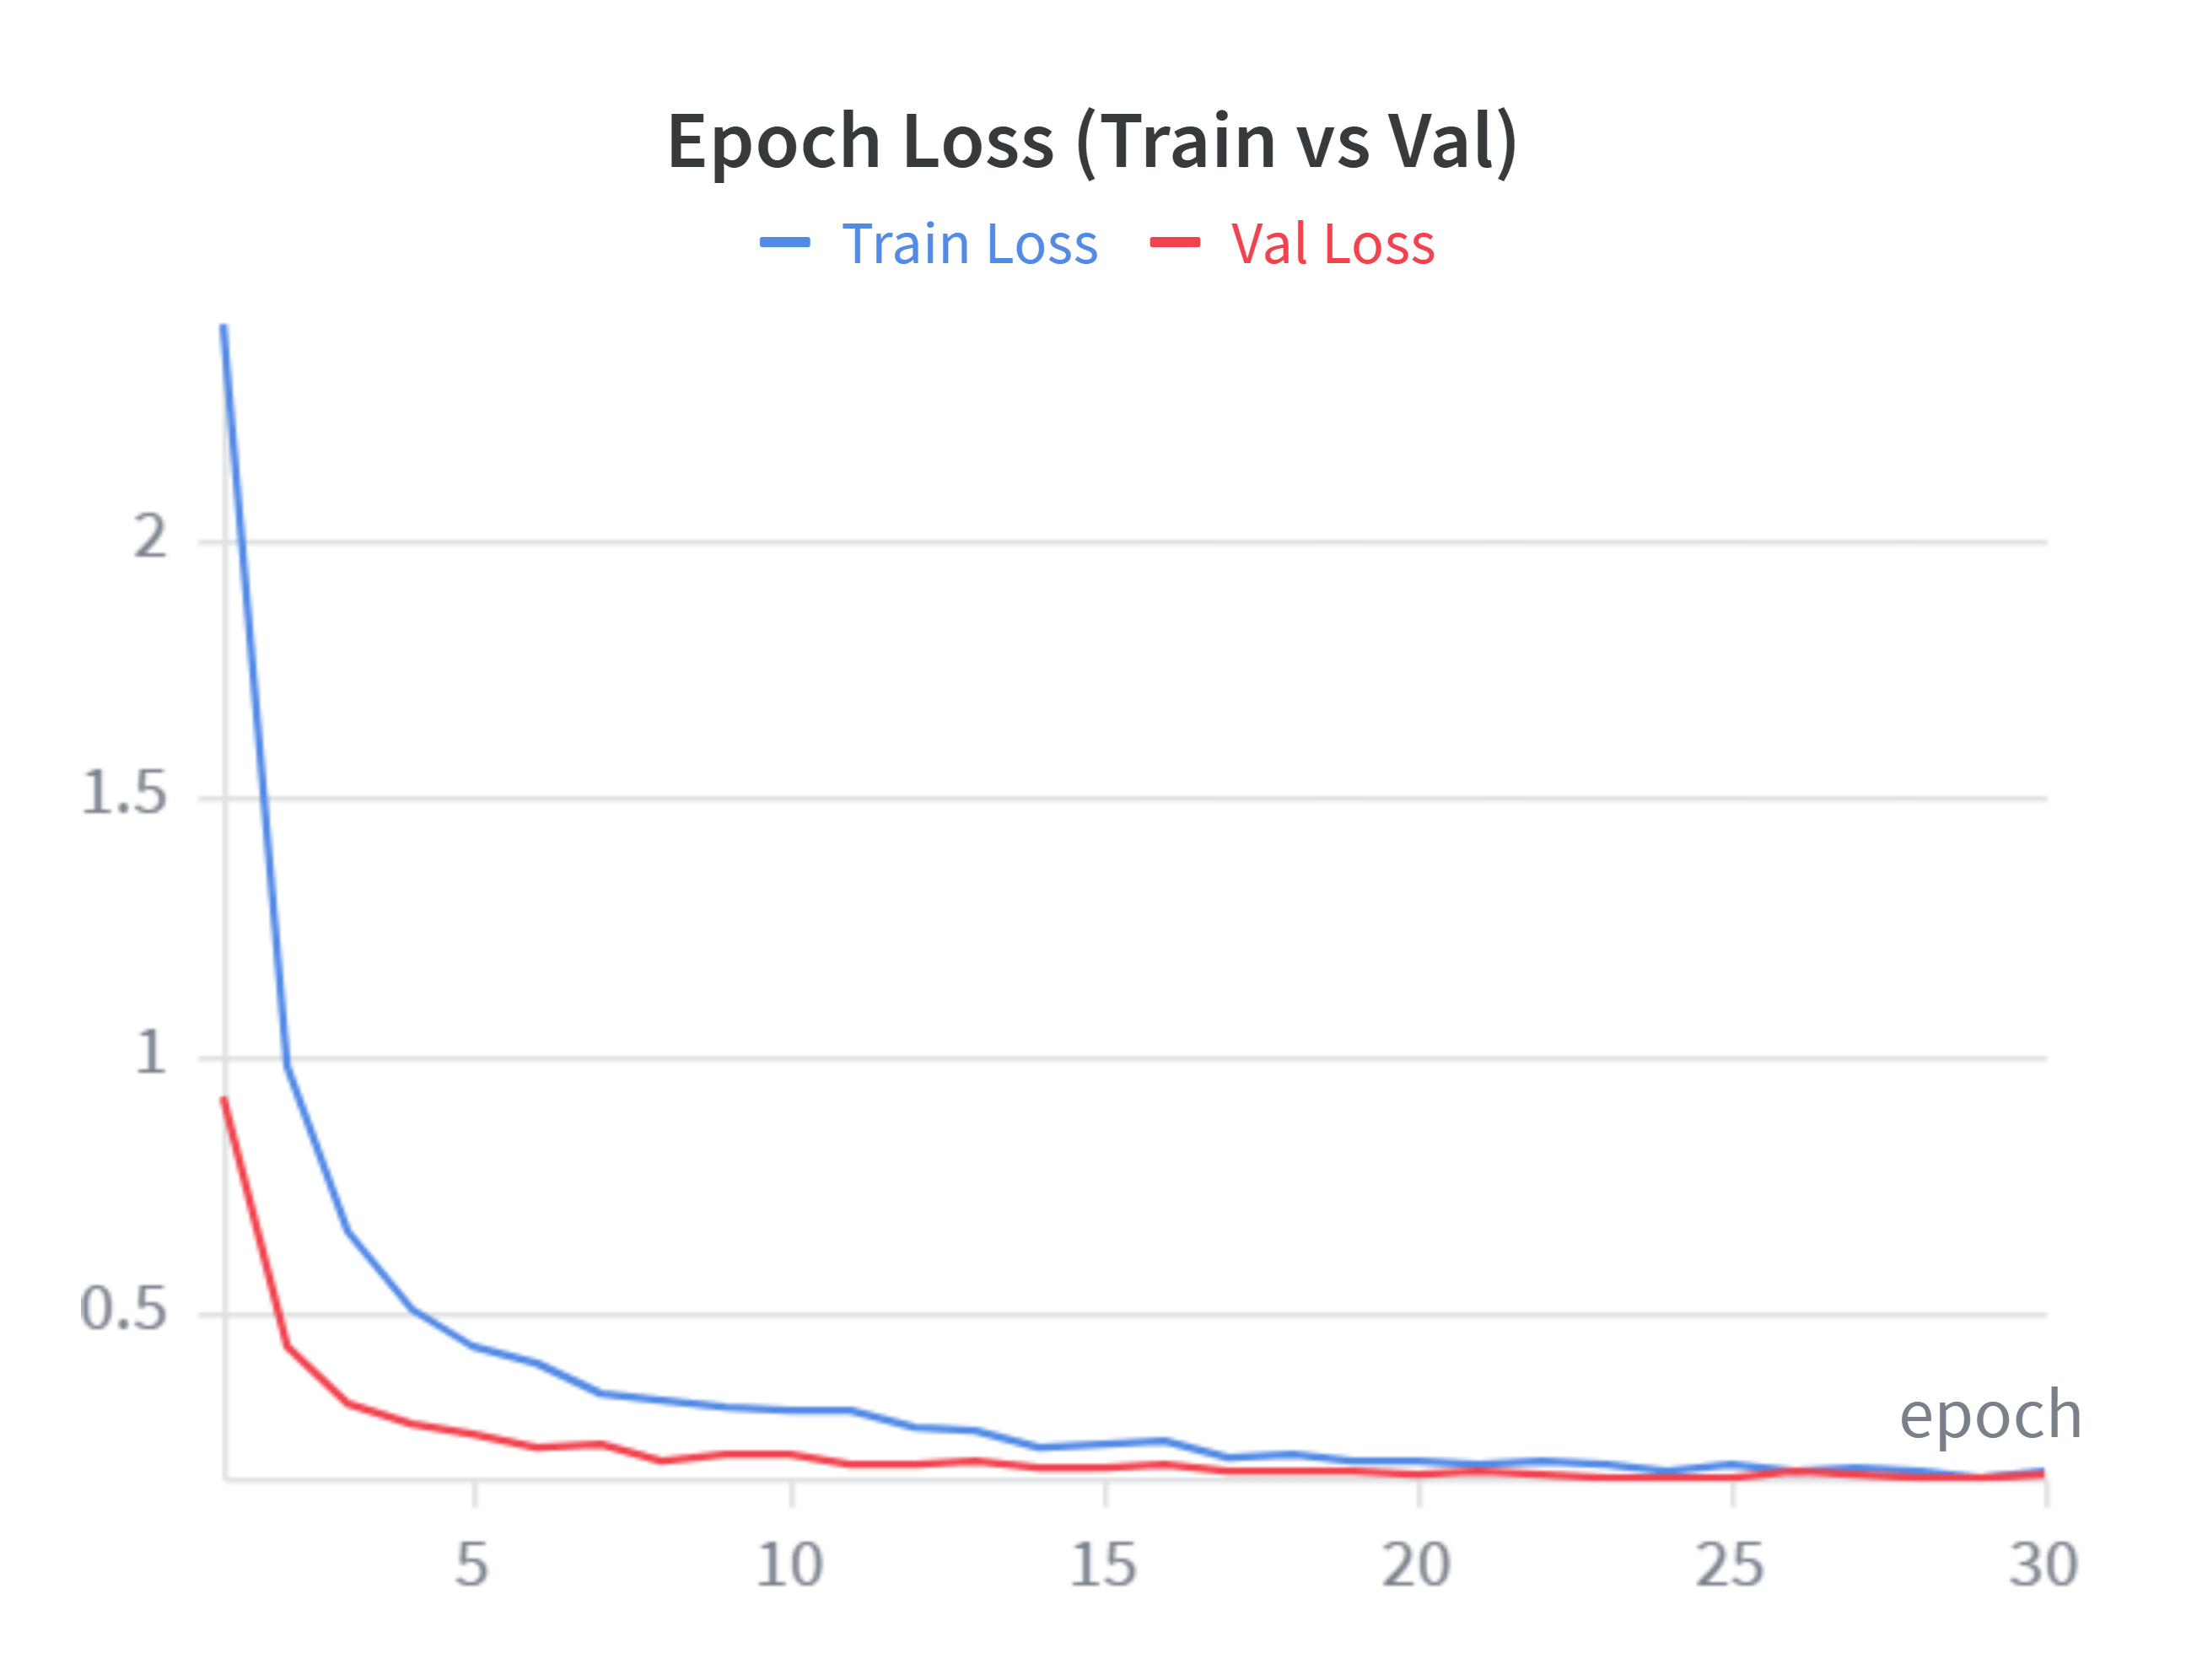
\includegraphics[width=\linewidth]{figures/task1/Epoch Loss.png}
        \caption{Epoch-level training and validation loss.}
    \end{subfigure}
    \hfill
    \begin{subfigure}{0.4\textwidth}
        \centering
        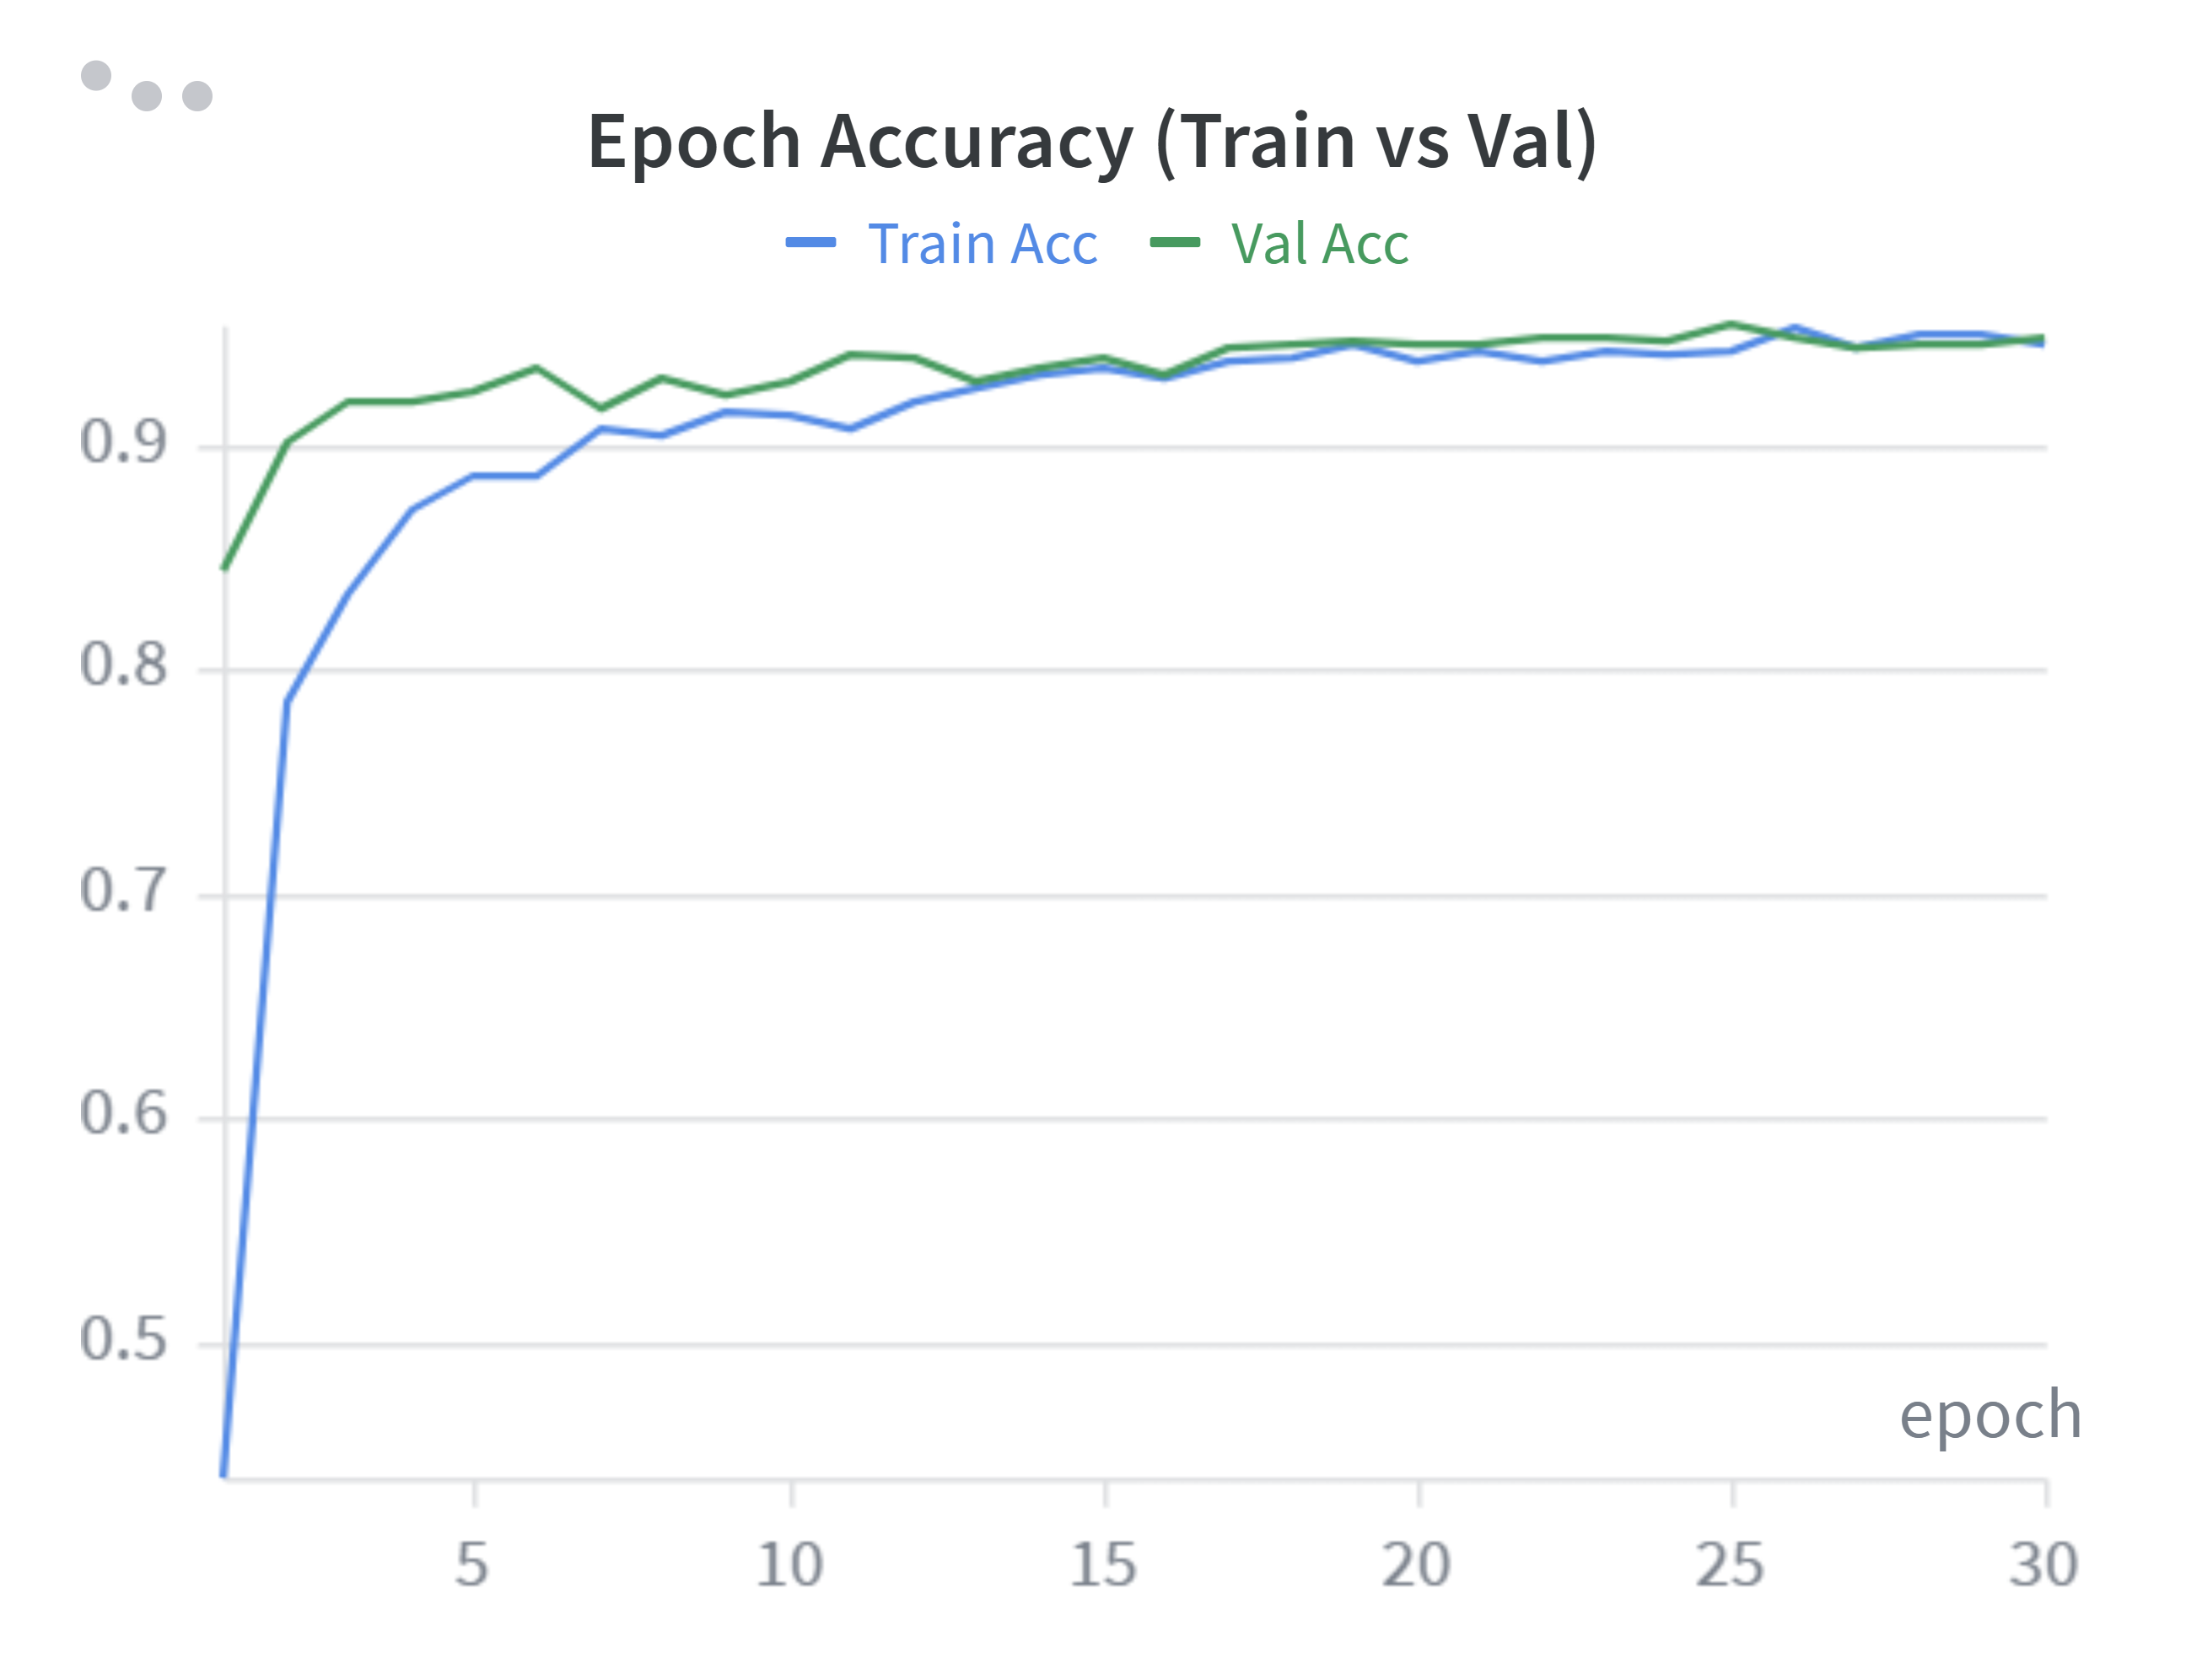
\includegraphics[width=\linewidth]{figures/task1/Epoch Acc.png}
        \caption{Epoch-level training and validation accuracy.}
    \end{subfigure}

    \vspace{0.5em}

    \begin{subfigure}{0.4\textwidth}
        \centering
        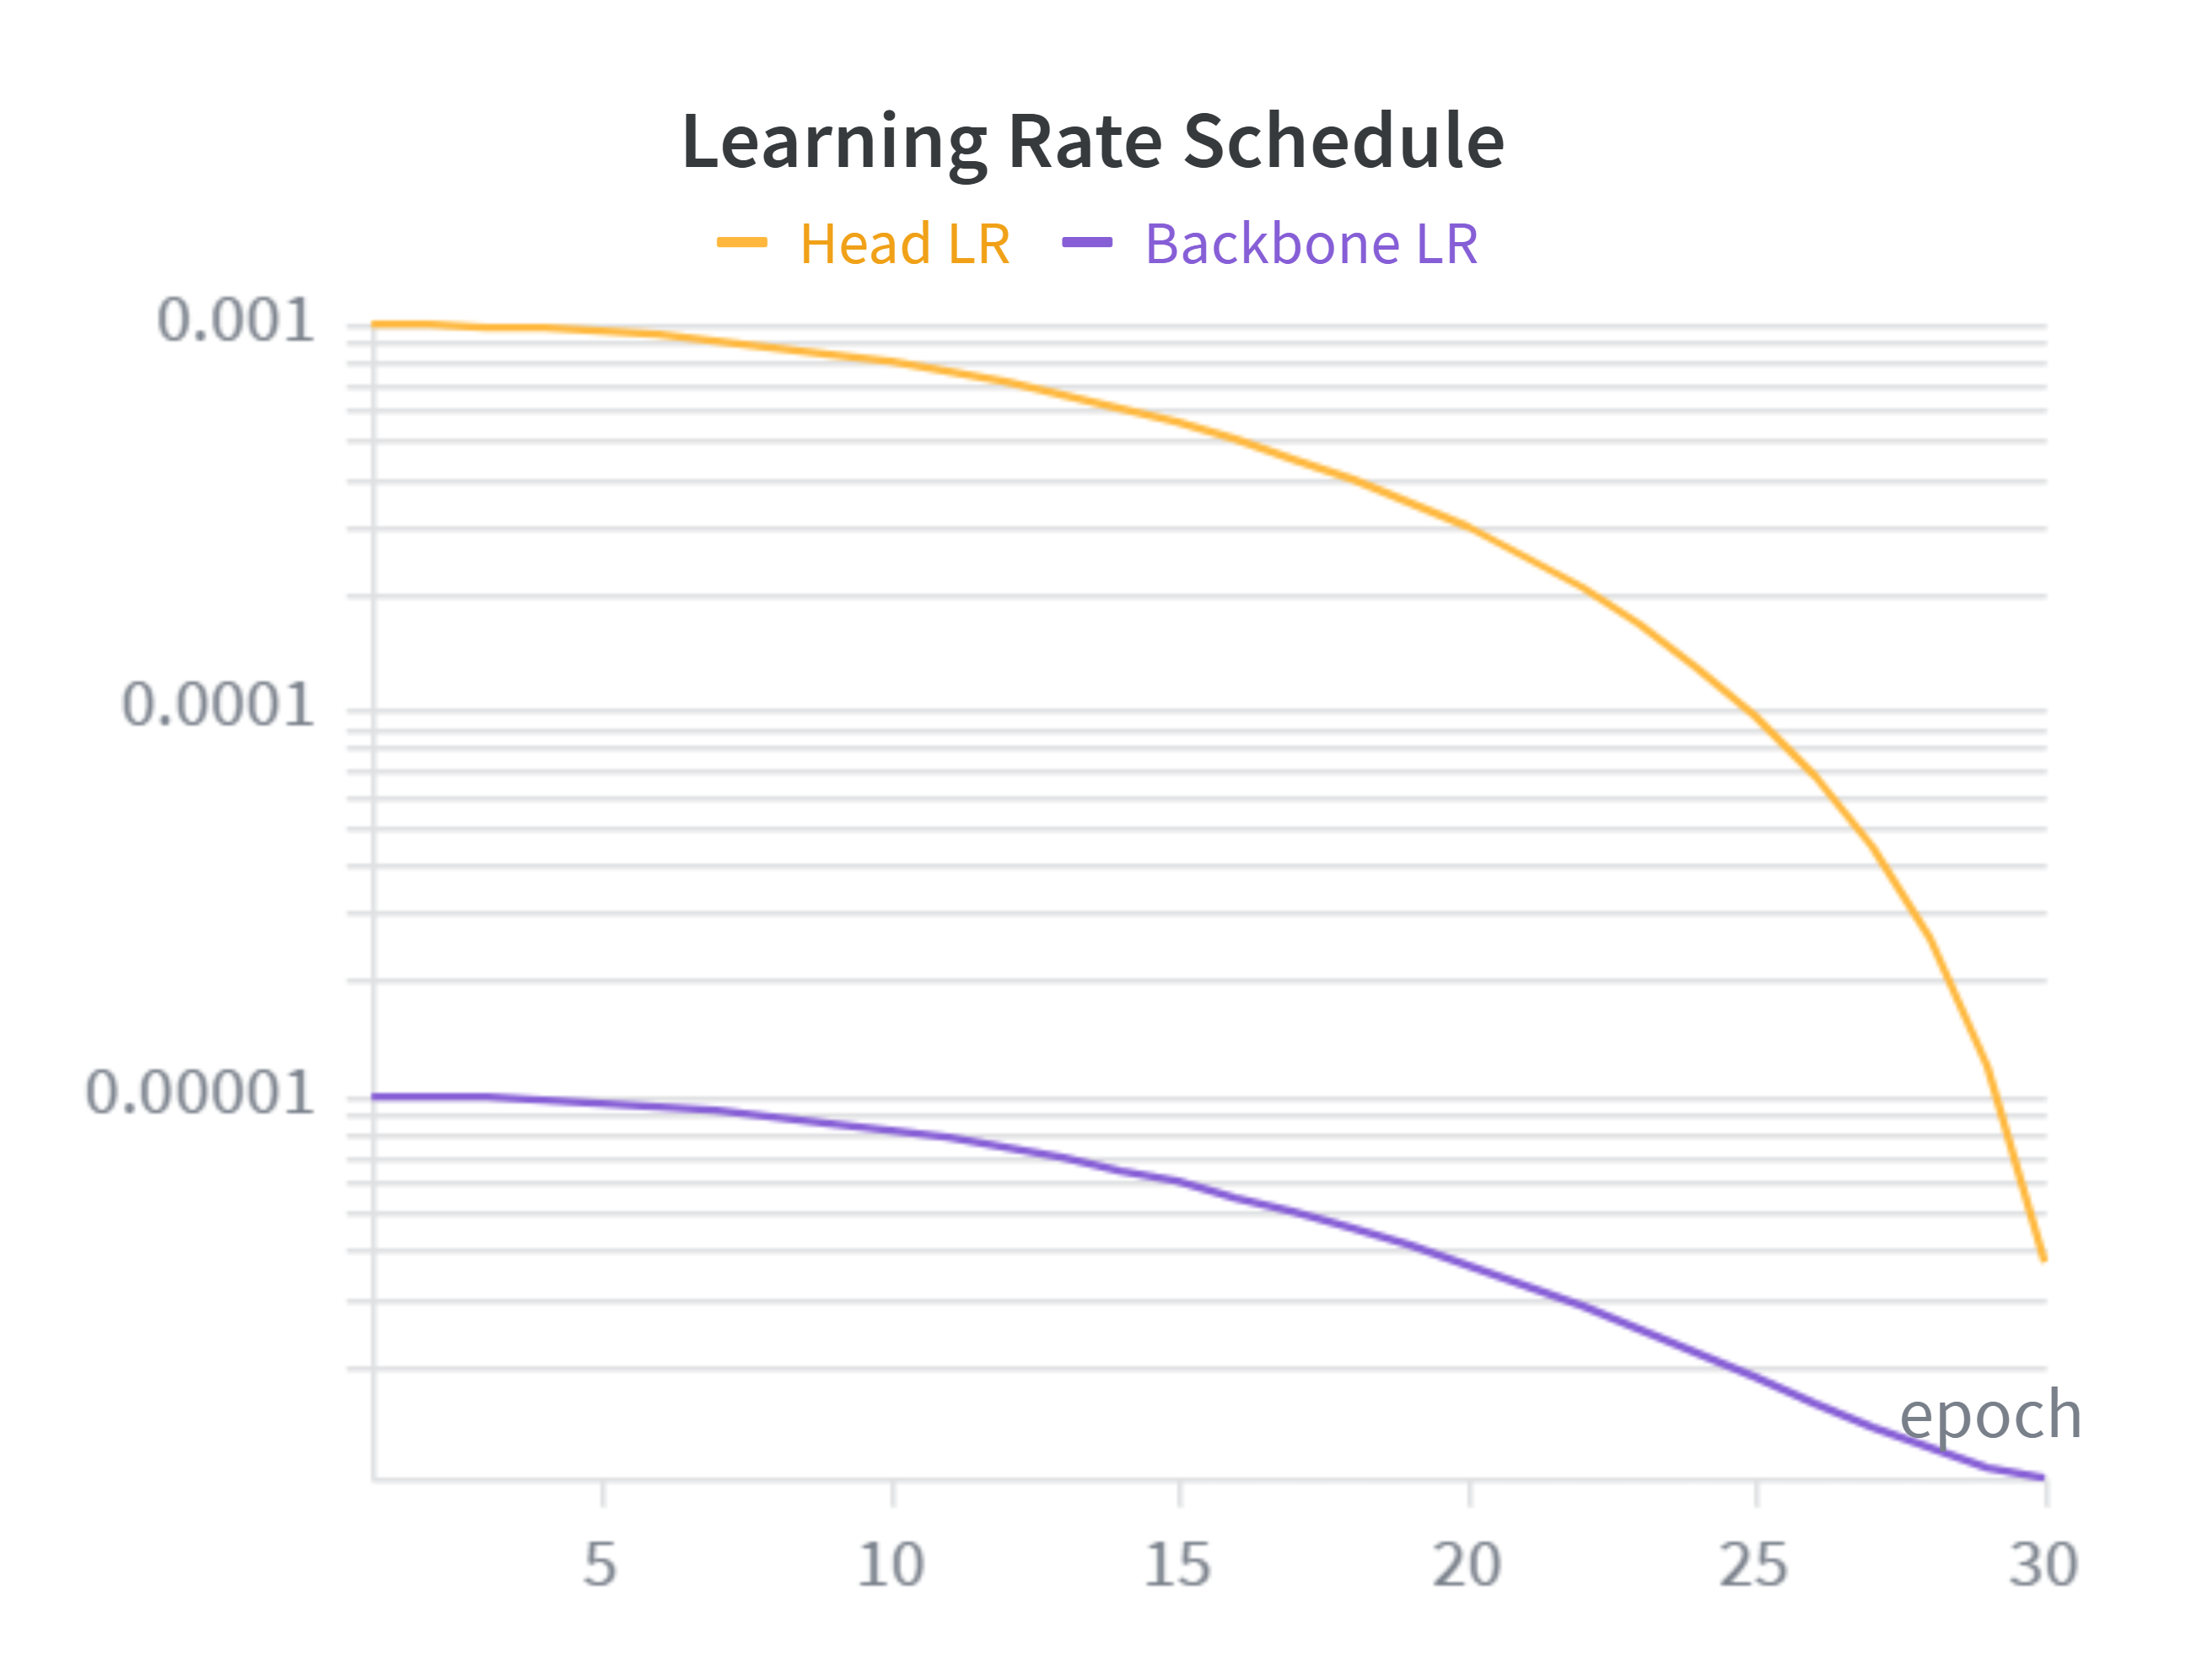
\includegraphics[width=\linewidth]{figures/task1/LR Schedule.png}
        \caption{Backbone and head learning rate schedules.}
    \end{subfigure}
    \hfill
    \begin{subfigure}{0.4\textwidth}
        \centering
        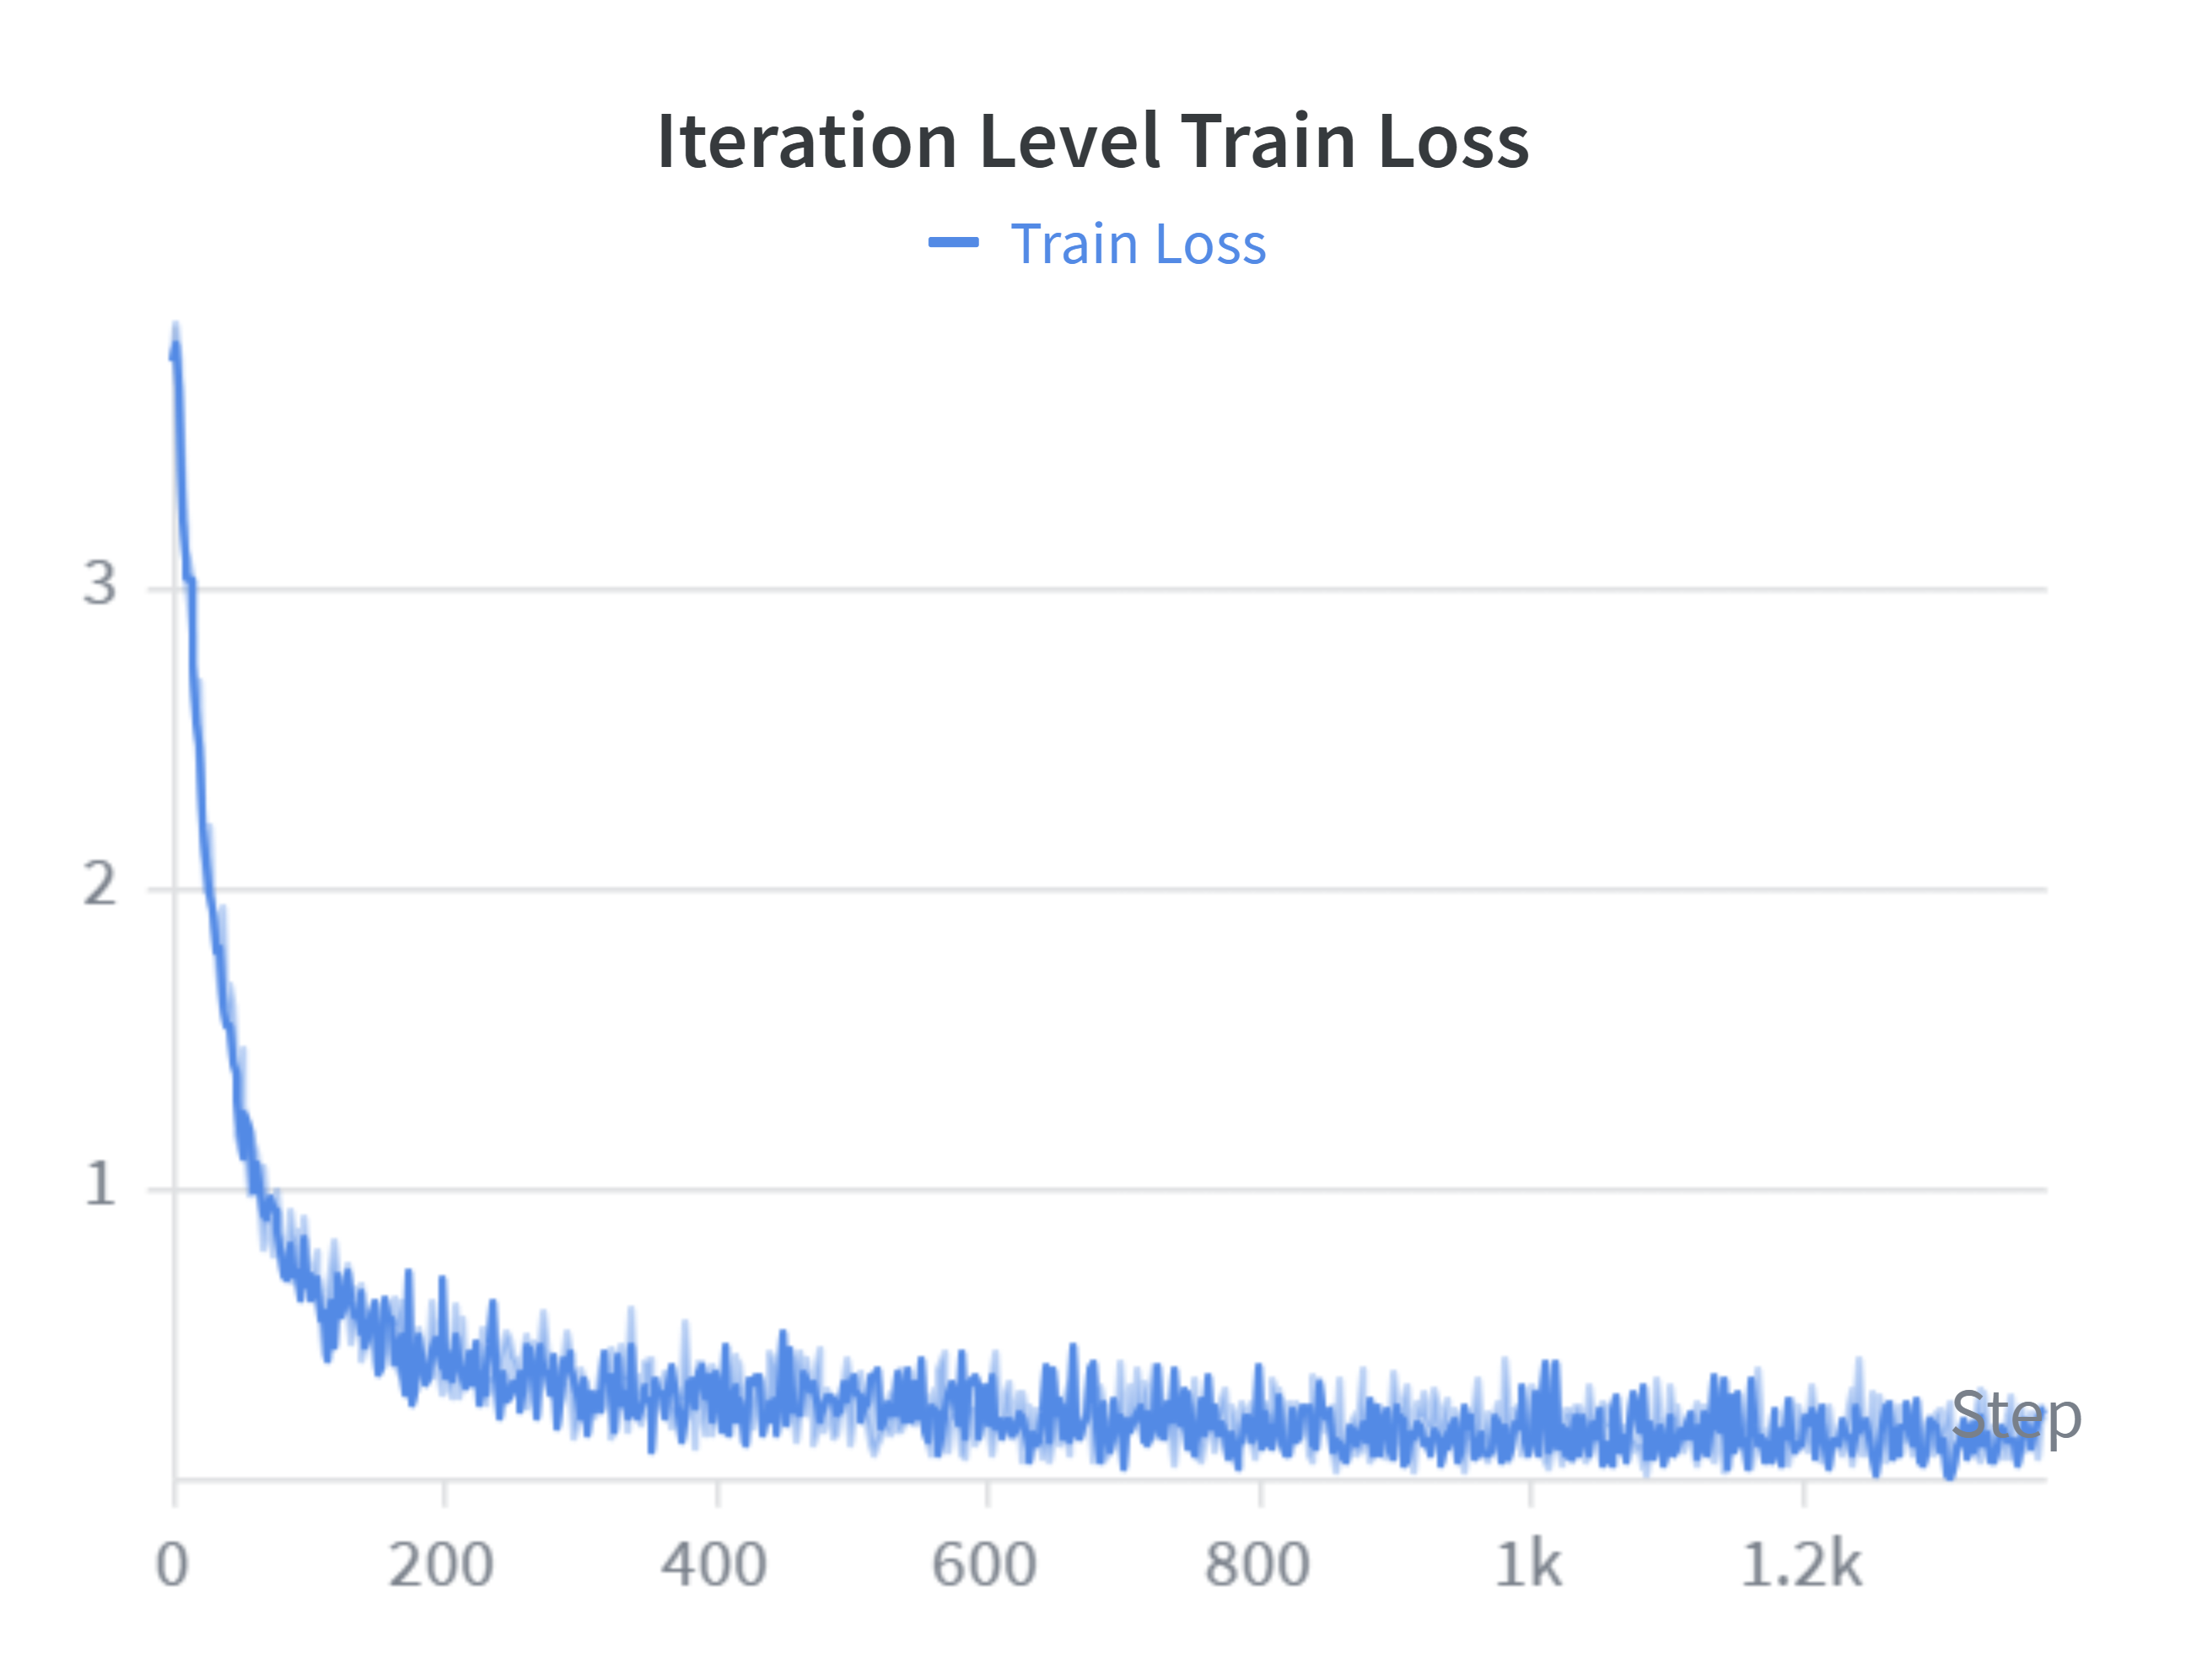
\includegraphics[width=\linewidth]{figures/task1/Iteration Train Loss.png}
        \caption{Iteration-level training loss.}
    \end{subfigure}

    \caption{Training dynamics of the final ResNet-34 configuration.}
    \label{fig:training_dynamics}
\end{figure}

As shown in Figure~\ref{fig:training_dynamics}(a), the training loss is initially higher than the validation loss due to strong data augmentation, especially random resized cropping and color jittering. As training proceeds, both losses gradually decrease and eventually converge to approximately 0.18 with only small oscillations near convergence.

A similar phenomenon can be observed in Figure~\ref{fig:training_dynamics}(b). The training accuracy is lower than the validation accuracy during early epochs, but the gap gradually disappears as optimization stabilizes. Both metrics eventually fluctuate around 95\%, indicating that the model achieves good generalization performance without severe overfitting.

Figure~\ref{fig:training_dynamics}(c) shows the cosine annealing learning rate schedule. The backbone learning rate remains consistently lower than the classification head learning rate throughout training, which helps preserve pretrained ImageNet features while allowing faster adaptation of the newly initialized classification head.

Finally, Figure~\ref{fig:training_dynamics}(d) presents the iteration-level training loss. Although mini-batch loss exhibits noticeable stochastic fluctuations, the overall downward trend remains stable throughout training.
